\documentclass{article}\usepackage[]{graphicx}\usepackage[]{xcolor}
% maxwidth is the original width if it is less than linewidth
% otherwise use linewidth (to make sure the graphics do not exceed the margin)
\makeatletter
\def\maxwidth{ %
  \ifdim\Gin@nat@width>\linewidth
    \linewidth
  \else
    \Gin@nat@width
  \fi
}
\makeatother

\definecolor{fgcolor}{rgb}{0.345, 0.345, 0.345}
\newcommand{\hlnum}[1]{\textcolor[rgb]{0.686,0.059,0.569}{#1}}%
\newcommand{\hlsng}[1]{\textcolor[rgb]{0.192,0.494,0.8}{#1}}%
\newcommand{\hlcom}[1]{\textcolor[rgb]{0.678,0.584,0.686}{\textit{#1}}}%
\newcommand{\hlopt}[1]{\textcolor[rgb]{0,0,0}{#1}}%
\newcommand{\hldef}[1]{\textcolor[rgb]{0.345,0.345,0.345}{#1}}%
\newcommand{\hlkwa}[1]{\textcolor[rgb]{0.161,0.373,0.58}{\textbf{#1}}}%
\newcommand{\hlkwb}[1]{\textcolor[rgb]{0.69,0.353,0.396}{#1}}%
\newcommand{\hlkwc}[1]{\textcolor[rgb]{0.333,0.667,0.333}{#1}}%
\newcommand{\hlkwd}[1]{\textcolor[rgb]{0.737,0.353,0.396}{\textbf{#1}}}%
\let\hlipl\hlkwb

\usepackage{framed}
\makeatletter
\newenvironment{kframe}{%
 \def\at@end@of@kframe{}%
 \ifinner\ifhmode%
  \def\at@end@of@kframe{\end{minipage}}%
  \begin{minipage}{\columnwidth}%
 \fi\fi%
 \def\FrameCommand##1{\hskip\@totalleftmargin \hskip-\fboxsep
 \colorbox{shadecolor}{##1}\hskip-\fboxsep
     % There is no \\@totalrightmargin, so:
     \hskip-\linewidth \hskip-\@totalleftmargin \hskip\columnwidth}%
 \MakeFramed {\advance\hsize-\width
   \@totalleftmargin\z@ \linewidth\hsize
   \@setminipage}}%
 {\par\unskip\endMakeFramed%
 \at@end@of@kframe}
\makeatother

\definecolor{shadecolor}{rgb}{.97, .97, .97}
\definecolor{messagecolor}{rgb}{0, 0, 0}
\definecolor{warningcolor}{rgb}{1, 0, 1}
\definecolor{errorcolor}{rgb}{1, 0, 0}
\newenvironment{knitrout}{}{} % an empty environment to be redefined in TeX

\usepackage{alltt}
\usepackage[margin=1.0in]{geometry} % To set margins
\usepackage{amsmath}  % This allows me to use the align functionality.
                      % If you find yourself trying to replicate
                      % something you found online, ensure you're
                      % loading the necessary packages!
\usepackage{amsfonts} % Math font
\usepackage{fancyvrb}
\usepackage{hyperref} % For including hyperlinks
\usepackage[shortlabels]{enumitem}% For enumerated lists with labels specified
                                  % We had to run tlmgr_install("enumitem") in R
\usepackage{float}    % For telling R where to put a table/figure
\usepackage{natbib}        %For the bibliography
\bibliographystyle{apalike}%For the bibliography
\IfFileExists{upquote.sty}{\usepackage{upquote}}{}
\begin{document}
\begin{enumerate}
%%%%%%%%%%%%%%%%%%%%%%%%%%%%%%%%%%%%%%%%%%%%%%%%%%%%%%%%%%%%%%%%%%%%%%%%%%%%%%%%
%%%%%%%%%%%%%%%%%%%%%%%%%%%%%%%%%%%%%%%%%%%%%%%%%%%%%%%%%%%%%%%%%%%%%%%%%%%%%%%%
% QUESTION 1
%%%%%%%%%%%%%%%%%%%%%%%%%%%%%%%%%%%%%%%%%%%%%%%%%%%%%%%%%%%%%%%%%%%%%%%%%%%%%%%%
%%%%%%%%%%%%%%%%%%%%%%%%%%%%%%%%%%%%%%%%%%%%%%%%%%%%%%%%%%%%%%%%%%%%%%%%%%%%%%%%
\item In Lab 3, you wrangled data from Essentia, Essentia models and LIWC. Rework your 
solution to Lab 3 using \texttt{tidyverse} \citep{tidyverse} instead of base \texttt{R}.
Specifically, rewrite your code for steps 1-4 of task 2 using \texttt{tidyverse} \citep{tidyverse}. 
Make sure to address any issues I noted in your code file, and ensure that your code 
runs in the directory as it is set up.
\begin{knitrout}\scriptsize
\definecolor{shadecolor}{rgb}{0.969, 0.969, 0.969}\color{fgcolor}\begin{kframe}
\begin{alltt}
\hlkwd{library}\hldef{(stringr)}
\hlkwd{library}\hldef{(jsonlite)}
\hlkwd{library}\hldef{(tidyverse)}

\hldef{filenames} \hlkwb{<-} \hlkwd{list.files}\hldef{(}\hlsng{"EssentiaOutput"}\hldef{)}
\hldef{json.indices} \hlkwb{<-} \hlkwd{which}\hldef{(}\hlkwd{str_count}\hldef{(filenames,} \hlkwc{pattern} \hldef{=} \hlsng{".json"}\hldef{)}\hlopt{==}\hlnum{1}\hldef{)}
\hldef{json.files} \hlkwb{<-} \hldef{filenames[json.indices]}
\hldef{len} \hlkwb{<-} \hlkwd{length}\hldef{(json.files)}

\hldef{df} \hlkwb{<-} \hlkwd{tibble}\hldef{(}
  \hlkwc{artist} \hldef{=} \hlkwd{character}\hldef{(len),}
  \hlkwc{album} \hldef{=} \hlkwd{character}\hldef{(len),}
  \hlkwc{track} \hldef{=} \hlkwd{character}\hldef{(len),}
  \hlkwc{`overall loudness`} \hldef{=} \hlkwd{numeric}\hldef{(len),}
  \hlkwc{`spectral energy`} \hldef{=} \hlkwd{numeric}\hldef{(len),}
  \hlkwc{dissonance} \hldef{=} \hlkwd{numeric}\hldef{(len),}
  \hlkwc{`pitch salience`} \hldef{=} \hlkwd{numeric}\hldef{(len),}
  \hlkwc{tempo} \hldef{=} \hlkwd{numeric}\hldef{(len),}
  \hlkwc{`beat loudness`} \hldef{=} \hlkwd{numeric}\hldef{(len),}
  \hlkwc{danceability} \hldef{=} \hlkwd{numeric}\hldef{(len),}
  \hlkwc{`tuning frequency`} \hldef{=} \hlkwd{numeric}\hldef{(len))}

\hlkwa{for}\hldef{(i} \hlkwa{in} \hlnum{1}\hlopt{:}\hlkwd{length}\hldef{(json.files))\{}
  \hldef{current.filename} \hlkwb{<-} \hldef{json.files[i]}
  \hldef{track.info} \hlkwb{<-} \hlkwd{str_split}\hldef{(}\hlkwd{str_sub}\hldef{(current.filename,} \hlkwc{end} \hldef{=} \hlopt{-}\hlnum{6}\hldef{),} \hlsng{"-"}\hldef{,} \hlkwc{simplify} \hldef{= T)}
  \hldef{track.path} \hlkwb{<-} \hlkwd{paste}\hldef{(}\hlsng{"EssentiaOutput/"}\hldef{,current.filename,} \hlkwc{sep} \hldef{=} \hlsng{""}\hldef{)} \hlcom{# track file path}
  \hldef{loaded.json} \hlkwb{<-} \hlkwd{fromJSON}\hldef{(track.path)}

  \hldef{df[i, ]} \hlkwb{<-} \hlkwd{tibble}\hldef{(}
    \hlkwc{artist} \hldef{= track.info[}\hlnum{1}\hldef{],}
    \hlkwc{album} \hldef{= track.info[}\hlnum{2}\hldef{],}
    \hlkwc{track} \hldef{= track.info[}\hlnum{3}\hldef{],}
    \hlkwc{overall_loudness} \hldef{= loaded.json}\hlopt{$}\hldef{lowlevel}\hlopt{$}\hldef{loudness_ebu128}\hlopt{$}\hldef{integrated,}
    \hlkwc{spectral_energy} \hldef{=} \hlkwd{unlist}\hldef{(loaded.json}\hlopt{$}\hldef{lowlevel}\hlopt{$}\hldef{spectral_energy),}
    \hlkwc{dissonance} \hldef{=} \hlkwd{unlist}\hldef{(loaded.json}\hlopt{$}\hldef{lowlevel}\hlopt{$}\hldef{dissonance),}
    \hlkwc{pitch_salience} \hldef{=} \hlkwd{unlist}\hldef{(loaded.json}\hlopt{$}\hldef{lowlevel}\hlopt{$}\hldef{pitch_salience),}
    \hlkwc{tempo} \hldef{= loaded.json}\hlopt{$}\hldef{rhythm}\hlopt{$}\hldef{bpm,}
    \hlkwc{beat_loudness} \hldef{=} \hlkwd{unlist}\hldef{(loaded.json}\hlopt{$}\hldef{rhythm}\hlopt{$}\hldef{beats_loudness),}
    \hlkwc{danceability} \hldef{=} \hlkwd{unlist}\hldef{(loaded.json}\hlopt{$}\hldef{rhythm}\hlopt{$}\hldef{danceability),}
    \hlkwc{tuning_frequency} \hldef{=} \hlkwd{unlist}\hldef{(loaded.json}\hlopt{$}\hldef{tonal}\hlopt{$}\hldef{tuning_frequency))}
\hldef{\}}
\hlcom{# view(df)}

\hldef{essentia.model} \hlkwb{<-} \hlkwd{read_csv}\hldef{(}\hlsng{"EssentiaOutput/EssentiaModelOutput.csv"}\hldef{)} \hlopt
  \hlkwd{mutate}\hldef{(}
    \hlkwc{valence} \hldef{=} \hlkwd{rowMeans}\hldef{(}\hlkwd{select}\hldef{(., deam_valence, emo_valence, muse_valence),} \hlkwc{na.rm} \hldef{= T),}
    \hlkwc{arousal} \hldef{=} \hlkwd{rowMeans}\hldef{(}\hlkwd{select}\hldef{(., deam_arousal, emo_arousal, muse_arousal),} \hlkwc{na.rm} \hldef{= T),}
    \hlkwc{aggressive} \hldef{=} \hlkwd{rowMeans}\hldef{(}\hlkwd{select}\hldef{(., eff_aggressive, nn_aggressive),} \hlkwc{na.rm} \hldef{= T),}
    \hlkwc{happy} \hldef{=} \hlkwd{rowMeans}\hldef{(}\hlkwd{select}\hldef{(., eff_happy, nn_happy),} \hlkwc{na.rm} \hldef{= T),}
    \hlkwc{party} \hldef{=} \hlkwd{rowMeans}\hldef{(}\hlkwd{select}\hldef{(., eff_party, nn_party),} \hlkwc{na.rm} \hldef{= T),}
    \hlkwc{relaxed} \hldef{=} \hlkwd{rowMeans}\hldef{(}\hlkwd{select}\hldef{(., eff_relax, nn_relax),} \hlkwc{na.rm} \hldef{= T),}
    \hlkwc{sad} \hldef{=} \hlkwd{rowMeans}\hldef{(}\hlkwd{select}\hldef{(., eff_sad, nn_sad),} \hlkwc{na.rm} \hldef{= T),}
    \hlkwc{acoustic} \hldef{=} \hlkwd{rowMeans}\hldef{(}\hlkwd{select}\hldef{(., eff_acoustic, nn_acoustic),} \hlkwc{na.rm} \hldef{= T),}
    \hlkwc{electric} \hldef{=} \hlkwd{rowMeans}\hldef{(}\hlkwd{select}\hldef{(., eff_electronic, nn_electronic),} \hlkwc{na.rm} \hldef{= T),}
    \hlkwc{instrumental} \hldef{=} \hlkwd{rowMeans}\hldef{(}\hlkwd{select}\hldef{(., eff_instrumental, nn_instrumental),} \hlkwc{na.rm} \hldef{= T),}
    \hlkwc{timbreBright} \hldef{= eff_timbre_bright) |>}
  \hlkwd{select}\hldef{(artist, album, track, valence, arousal, aggressive, happy, party,}
         \hldef{relaxed, sad, acoustic, electric, instrumental, timbreBright)}
\hlcom{# view(essentia.model)}

\hldef{liwc.output} \hlkwb{<-} \hlkwd{read_csv}\hldef{(}\hlsng{"LIWCOutput/LIWCOutput.csv"}\hldef{)}

\hldef{merged.output} \hlkwb{<-} \hldef{df |>}
  \hlkwd{left_join}\hldef{(essentia.model,} \hlkwc{by} \hldef{=} \hlkwd{c}\hldef{(}\hlsng{"artist"}\hldef{,}\hlsng{"album"}\hldef{,}\hlsng{"track"}\hldef{)) |>}
  \hlkwd{left_join}\hldef{(liwc.output,} \hlkwc{by} \hldef{=} \hlkwd{c}\hldef{(}\hlsng{"artist"}\hldef{,}\hlsng{"album"}\hldef{,}\hlsng{"track"}\hldef{)) |>}
  \hlkwd{rename}\hldef{(}\hlkwc{funct} \hldef{=} \hlsng{"function"}\hldef{)}
\hlcom{# view(merged.output)}

\hldef{training.data} \hlkwb{<-} \hlkwd{filter}\hldef{(merged.output, track} \hlopt{!=} \hlsng{"Allentown"}\hldef{)}
\hlkwd{write_csv}\hldef{(training.data,} \hlsng{"trainingdata.csv"}\hldef{)}
\hldef{testing.data} \hlkwb{<-} \hlkwd{filter}\hldef{(merged.output, track} \hlopt{==} \hlsng{"Allentown"}\hldef{)}
\hlkwd{write_csv}\hldef{(testing.data,} \hlsng{"testingdata.csv"}\hldef{)}
\hlcom{# view(training.data)}
\hlcom{# view(testing.data)}

\hlcom{# Spectral energy plot}
\hlkwd{ggplot}\hldef{(}\hlkwc{data} \hldef{= training.data)} \hlopt{+}
  \hlkwd{geom_boxplot}\hldef{(}\hlkwd{aes}\hldef{(}\hlkwc{x} \hldef{= artist,} \hlkwc{y} \hldef{= `spectral energy`))} \hlopt{+}
  \hlkwd{geom_hline}\hldef{(}\hlkwc{yintercept} \hldef{= testing.data}\hlopt{$}\hldef{`spectral energy`,}
             \hlkwc{color} \hldef{=} \hlsng{"orange"}\hldef{,} \hlkwc{linetype} \hldef{=} \hlsng{"dashed"}\hldef{,} \hlkwc{size} \hldef{=} \hlnum{1}\hldef{)} \hlopt{+}
  \hlkwd{theme_bw}\hldef{()} \hlopt{+}
  \hlkwd{xlab}\hldef{(}\hlsng{"Artist"}\hldef{)} \hlopt{+}
  \hlkwd{ylab}\hldef{(}\hlsng{"Spectral Energy"}\hldef{)} \hlopt{+}
  \hlkwd{labs}\hldef{(}\hlkwc{title} \hldef{=} \hlsng{"Comparison of Spectral Energy Values"}\hldef{,}
       \hlkwc{caption} \hldef{=} \hlsng{"Box plot of spectral energy between artists. Spectral energy of 'Allentown' in dashed orange."}\hldef{)} \hlopt{+}
  \hlkwd{theme}\hldef{(}\hlkwc{plot.title} \hldef{=} \hlkwd{element_text}\hldef{(}\hlkwc{hjust} \hldef{=} \hlnum{0.5}\hldef{),}
        \hlkwc{plot.caption} \hldef{=} \hlkwd{element_text}\hldef{(}\hlkwc{hjust} \hldef{=} \hlnum{0.5}\hldef{))}
\end{alltt}
\end{kframe}
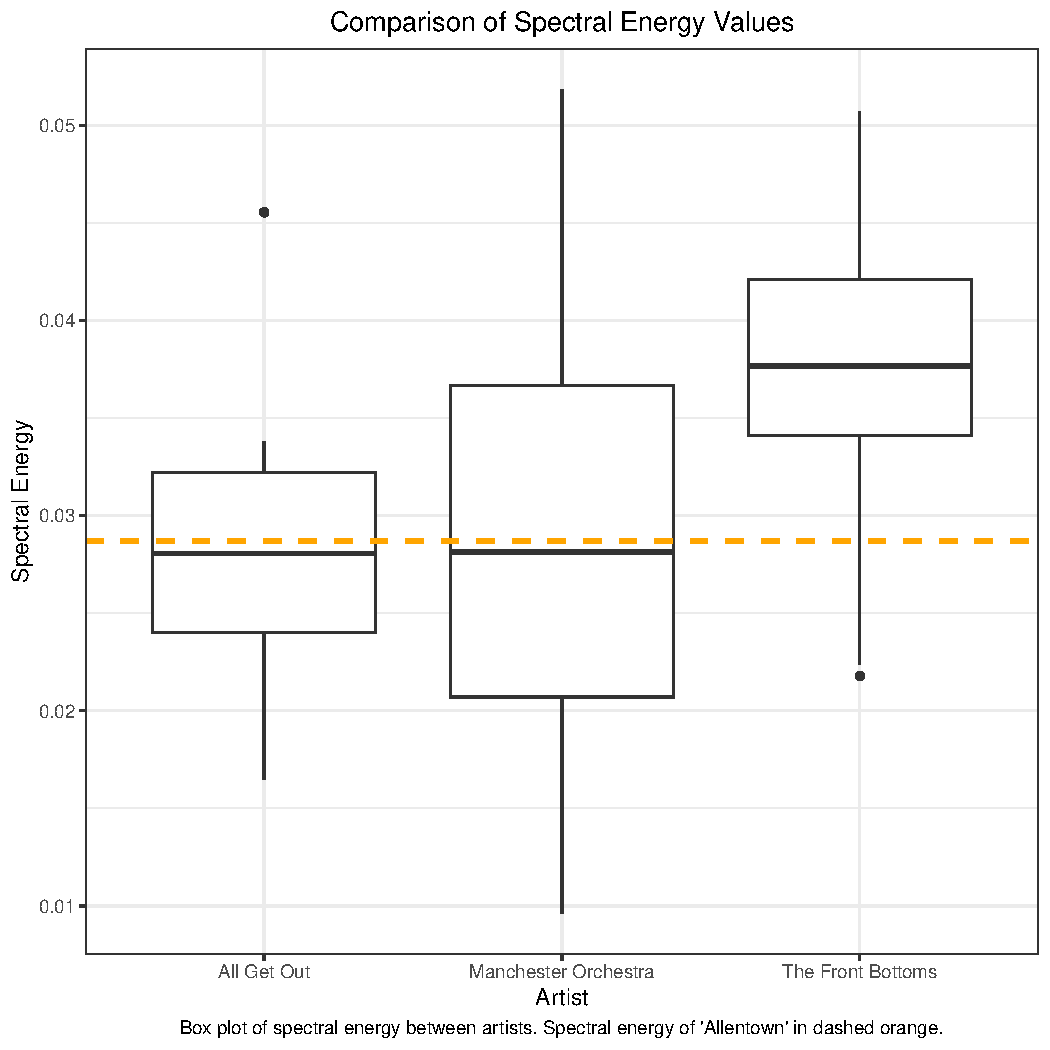
\includegraphics[width=\maxwidth]{figure/unnamed-chunk-1-1} 
\begin{kframe}\begin{alltt}
\hlcom{# Linguistic plot}
\hlkwd{ggplot}\hldef{(}\hlkwc{data} \hldef{= training.data)} \hlopt{+}
  \hlkwd{geom_boxplot}\hldef{(}\hlkwd{aes}\hldef{(}\hlkwc{x} \hldef{= artist,} \hlkwc{y} \hldef{= Linguistic))} \hlopt{+}
  \hlkwd{geom_hline}\hldef{(}\hlkwc{yintercept} \hldef{= testing.data}\hlopt{$}\hldef{Linguistic,}
             \hlkwc{color} \hldef{=} \hlsng{"orange"}\hldef{,} \hlkwc{linetype} \hldef{=} \hlsng{"dashed"}\hldef{,} \hlkwc{size} \hldef{=} \hlnum{1}\hldef{)} \hlopt{+}
  \hlkwd{theme_bw}\hldef{()} \hlopt{+}
  \hlkwd{xlab}\hldef{(}\hlsng{"Artist"}\hldef{)} \hlopt{+}
  \hlkwd{ylab}\hldef{(}\hlsng{"Linguistic Value"}\hldef{)} \hlopt{+}
  \hlkwd{labs}\hldef{(}\hlkwc{title} \hldef{=} \hlsng{"Comparison of Linguistic Values"}\hldef{,}
       \hlkwc{caption} \hldef{=} \hlsng{"Box plot of linguistic value between artists. Linguistic value of 'Allentown' in dashed orange."}\hldef{)} \hlopt{+}
  \hlkwd{theme}\hldef{(}\hlkwc{plot.title} \hldef{=} \hlkwd{element_text}\hldef{(}\hlkwc{hjust} \hldef{=} \hlnum{0.5}\hldef{),}
        \hlkwc{plot.caption} \hldef{=} \hlkwd{element_text}\hldef{(}\hlkwc{hjust} \hldef{=} \hlnum{0.5}\hldef{))}
\end{alltt}
\end{kframe}
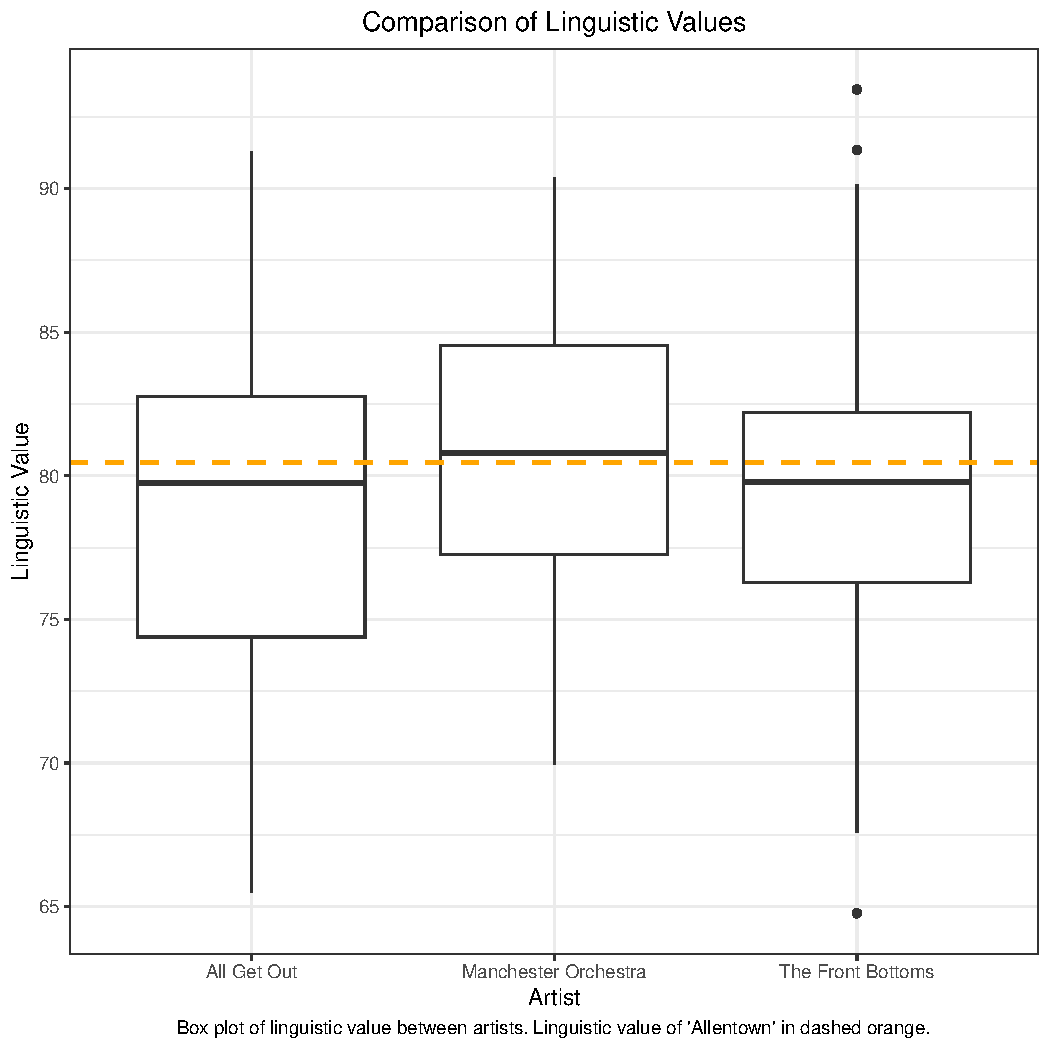
\includegraphics[width=\maxwidth]{figure/unnamed-chunk-1-2} 
\end{knitrout}
\end{enumerate}
\bibliography{bibliography}
\end{document}
